% ---------
% Preamble.
% ---------

% Document type.
\documentclass{article}

% Import custom style.
\usepackage{../.preamble/tikz_diagrams_template}

% Color theme (black, red, blue, green, orange, purple, gold).
\colortheme{blue}

% ---------
% Document.
% ---------

\begin{document}

    % -----------------
    % TikZ environment.
    % -----------------

    \begin{tikzpicture}

        % -----------------
        % Airplane drawing.
        % -----------------
        
        \node[anchor=south west,inner sep=0] (image) at (0,0) {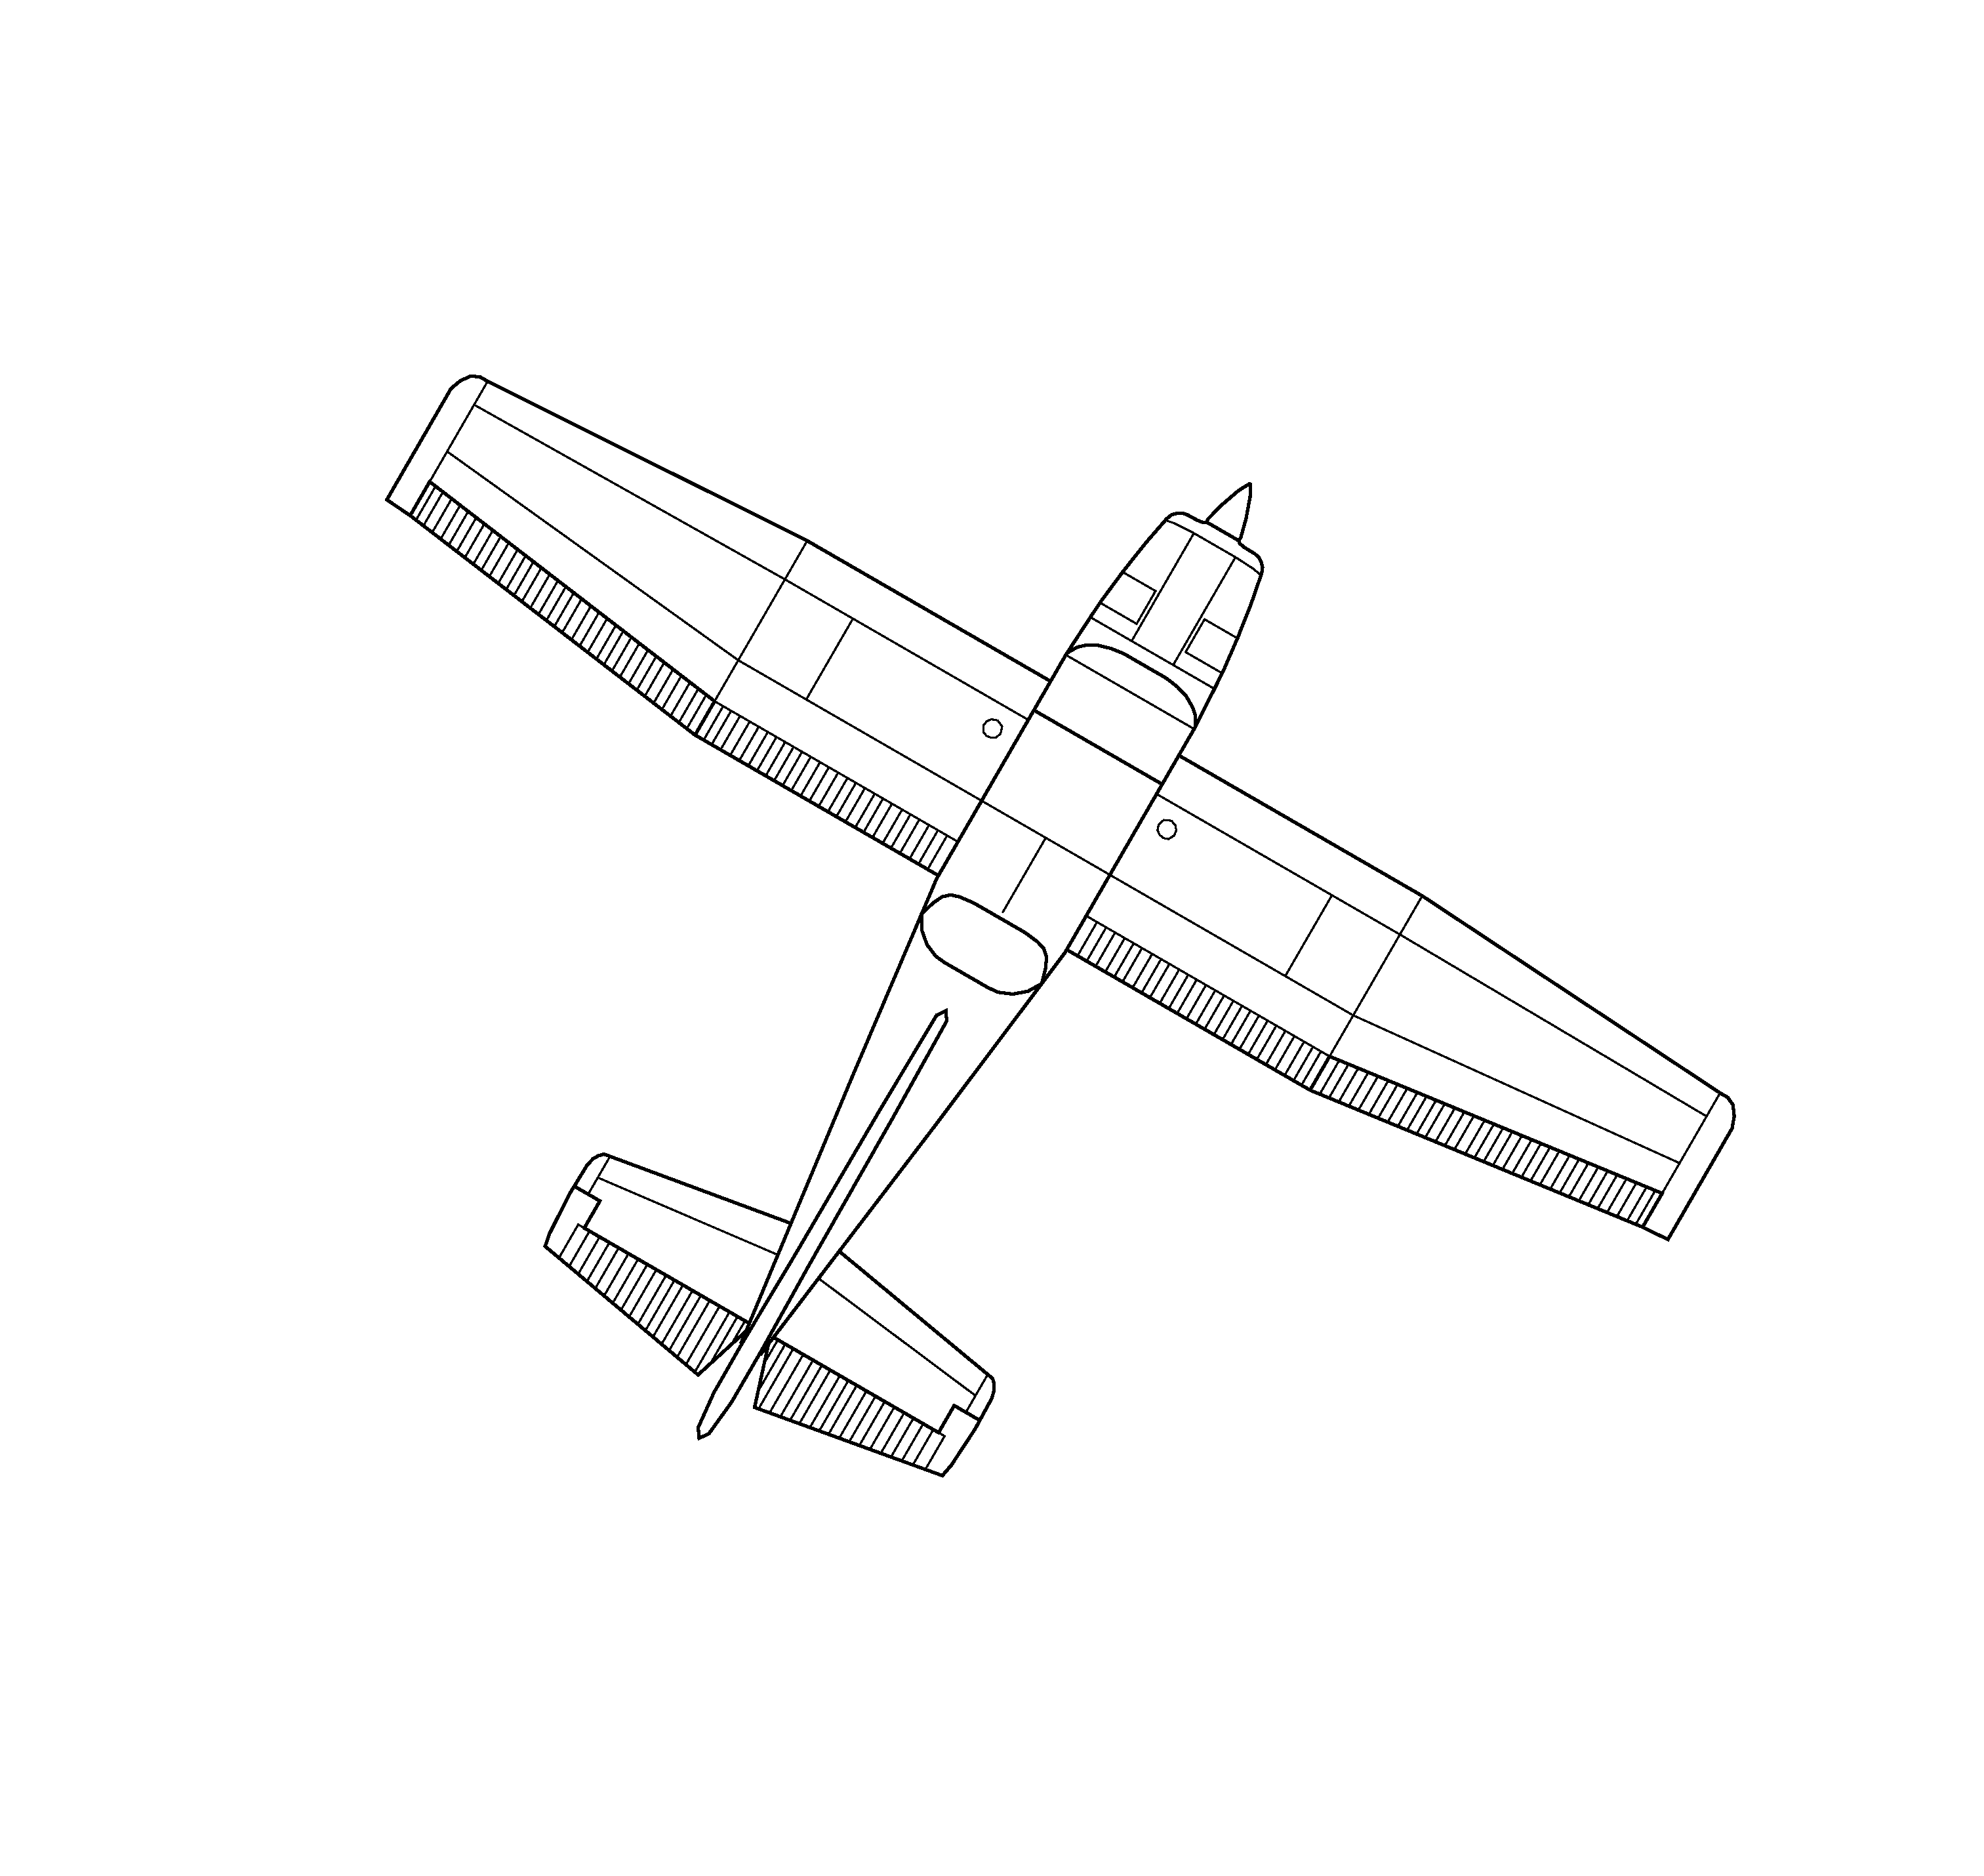
\includegraphics[width=0.6\textwidth]{../.images/airplane_yaw.eps}};

        % -----------
        % Parameters.
        % -----------
        
        % Origin.
        \pgfmathsetmacro{\Ox}{5.3}
        \pgfmathsetmacro{\Oy}{5.3}

        % pitch angle [deg]
        \pgfmathsetmacro{\yawangle}{30}
        
        % Axes length.
        \pgfmathsetmacro{\axlen}{5}

        % arc radius
        \pgfmathsetmacro{\arcrad}{0.9*\axlen}

        % -----------
        % Body frame.
        % -----------
        
        % xb-axis endpoint
        \pgfmathsetmacro{\xbx}{\Ox+sin(\yawangle)*\axlen}
        \pgfmathsetmacro{\xby}{\Oy+cos(\yawangle)*\axlen}

        % yb-axis endpoint
        \pgfmathsetmacro{\ybx}{\Ox+cos(\yawangle)*\axlen}
        \pgfmathsetmacro{\yby}{\Oy-sin(\yawangle)*\axlen}

        % Body axes.
        \draw[line width=0.5mm](\Ox,\Oy)--(\xbx,\xby)node[pos=1.04]{$x_{b}$};
        \draw[line width=0.5mm](\Ox,\Oy)--(\ybx,\yby)node[pos=1.06]{$y_{b}$};

        % ------------
        % World frame.
        % ------------
        
        % xw-axis endpoint
        \pgfmathsetmacro{\xwx}{\Ox}
        \pgfmathsetmacro{\xwy}{\Oy+\axlen}

        % yw-axis endpoint
        \pgfmathsetmacro{\ywx}{\Ox+\axlen}
        \pgfmathsetmacro{\ywy}{\Oy}

        % World axes.
        \draw[dotted,line width=0.5mm](\Ox,\Oy)--(\xwx,\xwy)node[pos=1.04]{$x_{w}$};
        \draw[dotted,line width=0.5mm](\Ox,\Oy)--(\ywx,\ywy)node[pos=1.06]{$y_{w}$};

        % ----------
        % Yaw angle.
        % ----------

        % arrow 1 starting point
        \pgfmathsetmacro{\arcxa}{\Ox}
        \pgfmathsetmacro{\arcya}{\Oy+\arcrad}

        % arrow 1
        \draw[-mylatex',color_theme,thick](\arcxa,\arcya)arc(90:60:\arcrad)node[midway,above,yshift=2]{$\psi_{\mathrm{world}\to\mathrm{body}}$};

        % arrow 2 starting point
        \pgfmathsetmacro{\arcxb}{\Ox+\arcrad}
        \pgfmathsetmacro{\arcyb}{\Oy}

        % arrow 2
        \draw[-mylatex',color_theme,thick](\arcxb,\arcyb)arc(0:-30:\arcrad)node[midway,right]{$\psi_{\mathrm{world}\to\mathrm{body}}$};
        
    \end{tikzpicture}

\end{document}